\documentclass[UTF8,fontset=none,12pt]{ctexart}

\setCJKmainfont{Songti SC}
\setCJKsansfont{PingFang SC}
\setCJKmonofont{Songti SC}

\usepackage[a4paper,margin=2.35cm]{geometry}
\usepackage{amsmath,amssymb,amsthm,mathtools,bm}
\usepackage{graphicx}
\usepackage{float}
\usepackage{booktabs}
\usepackage{enumitem}
\usepackage[hidelinks]{hyperref}

\newcommand{\C}{\mathbb{C}}
\newcommand{\R}{\mathbb{R}}
\newcommand{\range}{\operatorname{range}}
\newcommand{\nullspace}{\operatorname{null}}
\newcommand{\rank}{\operatorname{rank}}
\theoremstyle{definition}
\newtheorem{theorem}{定理}
\renewcommand{\thetheorem}{8.\arabic{theorem}}

\title{数值线性代数\quad 第 8 讲：Gram--Schmidt 正交化}
\author{Lloyd N. Trefethen、David Bau III\quad 中文阅读版}
\date{}

\begin{document}
\maketitle
\pagestyle{plain}

Gram--Schmidt 迭代是计算 QR 分解的两种主要数值算法之一.它通过一系列矩阵运算把矩阵的列变成标准正交列.这些运算还可以理解为在矩阵右侧乘以上三角矩阵，因此本讲也把它称为\textbf{三角正交化}.

\section*{Gram--Schmidt 投影}

上一讲以经典形式介绍了 Gram--Schmidt 迭代.现在我们用正交投影重新描述同一个算法.设 $A\in\C^{m\times n}$，$m\ge n$，$A$ 满列秩，列向量为 $\{a_j\}$.定义一列正交投影 $P_j$，并令
\begin{equation}
    q_1=\frac{P_1a_1}{\|P_1a_1\|_2},\qquad
    q_2=\frac{P_2a_2}{\|P_2a_2\|_2},\qquad\cdots\qquad
    q_n=\frac{P_na_n}{\|P_na_n\|_2}.
    \tag{8.1}
\end{equation}
其中，$P_j$ 是秩为 $m-(j-1)$ 的 $m\times m$ 正交投影，把 $\C^m$ 正交投影到与 $q_1,\ldots,q_{j-1}$ 都正交的空间.当 $j=1$ 时，这个定义就是单位矩阵 $P_1=I$.

按式 (8.1) 定义的 $q_j$ 与 $q_1,\ldots,q_{j-1}$ 正交，属于 $\langle a_1,\ldots,a_j\rangle$，且范数为 1.因此，式 (8.1) 与式 (7.6)--(7.8) 等价，也就与算法 7.1 等价.

正交投影 $P_j$ 可以显式写出.令 $\widehat Q_{j-1}$ 表示包含 $Q$ 前 $j-1$ 列的 $m\times(j-1)$ 矩阵：
\begin{equation}
    \widehat Q_{j-1}=[q_1\ \ q_2\ \ \cdots\ \ q_{j-1}].
    \tag{8.2}
\end{equation}
那么
\begin{equation}
    P_j=I-\widehat Q_{j-1}\widehat Q_{j-1}^*.
    \tag{8.3}
\end{equation}
读者现在应该可以直接看出，式 (8.3) 正是式 (7.5) 中作用于 $a_j$ 的算子.

\section*{修改后的 Gram--Schmidt 算法}

实际计算中，我们不会像算法 7.1 和式 (8.1) 那样直接应用 Gram--Schmidt 公式，因为这样的计算顺序数值上不稳定.幸运的是，只需做一个简单修改就能改善这一点.这里先把“稳定”理解为：算法对计算机舍入误差的影响不太敏感；数值稳定性将在下一讲以及第 14 讲开始系统讨论.

对每个 $j$，算法 7.1 计算一次秩为 $m-(j-1)$ 的正交投影：
\begin{equation}
    v_j=P_ja_j.
    \tag{8.4}
\end{equation}
相比之下，修改后的 Gram--Schmidt 算法用 $j-1$ 次秩为 $m-1$ 的投影得到同一个结果.回忆式 (6.9)：对非零向量 $q\in\C^m$，$P_{\perp q}$ 表示投影到 $q$ 的正交补上的秩 $m-1$ 正交投影.根据 $P_j$ 的定义，有
\begin{equation}
    P_j=P_{\perp q_{j-1}}\cdots P_{\perp q_2}P_{\perp q_1},
    \tag{8.5}
\end{equation}
其中仍约定 $P_1=I$.因此，式 (8.4) 等价于
\begin{equation}
    v_j=P_{\perp q_{j-1}}\cdots P_{\perp q_2}P_{\perp q_1}a_j.
    \tag{8.6}
\end{equation}
修改后的 Gram--Schmidt 算法正是用式 (8.6) 代替式 (8.4).

从数学上看，式 (8.6) 与式 (8.4) 等价；但它们对应的算术运算顺序不同.修改后的算法按顺序计算
\begin{equation}
\begin{aligned}
    v_j^{(1)}&=a_j,\\
    v_j^{(2)}&=P_{\perp q_1}v_j^{(1)}
        =v_j^{(1)}-q_1q_1^*v_j^{(1)},\\
    v_j^{(3)}&=P_{\perp q_2}v_j^{(2)}
        =v_j^{(2)}-q_2q_2^*v_j^{(2)},\\
    &\ \vdots\\
    v_j=v_j^{(j)}&=P_{\perp q_{j-1}}v_j^{(j-1)}
        =v_j^{(j-1)}-q_{j-1}q_{j-1}^*v_j^{(j-1)}.
\end{aligned}
\tag{8.7}
\end{equation}
在有限精度的计算机算术中，式 (8.7) 产生的误差比式 (8.4) 更小.实现时，一旦 $q_i$ 已知，就可以对所有 $j>i$ 立即把投影 $P_{\perp q_i}$ 作用到 $v_j^{(i)}$ 上.

\subsection*{算法 8.1：修改后的 Gram--Schmidt}

\begin{verbatim}
for i = 1 to n
    v_i = a_i
for i = 1 to n
    r_ii = ||v_i||_2
    q_i = v_i / r_ii
    for j = i+1 to n
        r_ij = q_i^* v_j
        v_j = v_j - r_ij q_i
\end{verbatim}

实践中通常让 $v_i$ 覆盖原来的 $a_i$，让 $q_i$ 覆盖原来的 $v_i$，以节省存储空间.读者可以对照算法 7.1 和算法 8.1，直到确信它们等价为止.

\section*{运算量}

Gram--Schmidt 算法是本书介绍的第一个算法.对于任何算法，评估其代价都很重要.本书采用经典方式，计算算法需要的浮点运算次数（\textbf{flops}）.每次加、减、乘、除或平方根都计为一次 flop.这里不区分实数和复数运算，尽管在大多数计算机上两者的实际代价差别很大.

此外，算法代价不只由运算次数决定.单处理器上，执行时间还受数据在存储层次各部分之间移动以及其他任务竞争的影响；多处理器上，处理器之间的通信有时比实际计算更重要.本书有意保持经典风格，聚焦算法基础，暂时忽略这些因素.

对于两种 Gram--Schmidt 迭代，有如下经典结果.

\begin{theorem}
算法 7.1 和算法 8.1 计算一个 $m\times n$ 矩阵的 QR 分解时，所需浮点运算次数的主项为 $\sim 2mn^2$ flops.
\end{theorem}

这里的定理只表达 flops 计数的主导项.符号 $\sim$ 的通常渐近含义是
\[
    \lim_{m,n\to\infty}
    \frac{\text{浮点运算次数}}{2mn^2}=1.
\]
讨论算法运算量时，通常会像这里一样舍弃低阶项；除非 $m,n$ 很小，否则它们往往不重要.

下面以修改后的 Gram--Schmidt 算法为例说明.当 $m,n$ 很大时，运算量主要来自内层循环：
\[
    r_{ij}=q_i^*v_j,\qquad v_j=v_j-r_{ij}q_i.
\]
第一行计算内积 $q_i^*v_j$，需要 $m$ 次乘法和 $m-1$ 次加法；第二行计算 $v_j-r_{ij}q_i$，需要 $m$ 次乘法和 $m$ 次减法.所以每次内层迭代约需 $4m$ flops，即每个列向量元素需要 4 次 flop.总运算量渐近为
\begin{equation}
    \sum_{i=1}^{n}\sum_{j=i+1}^{n}4m
    =\sum_{i=1}^{n}(n-i)4m
    \sim 2mn^2.
    \tag{8.8}
\end{equation}

\section*{从几何图形计算运算量}

运算量当然可以像式 (8.8) 那样代数计算，这也是数值分析文献中的标准做法.不过，换一条几何路径得到同样结论也很有启发性.

在算法 8.1 外层循环的第一步，算法作用于整个矩阵，从其他列中减去列 1 的倍数；第二步作用于一个子矩阵，从第 3 列到第 $n$ 列中减去列 2 的倍数.如此继续，每一步的列维数都减少 1，直到最后一步只修改第 $n$ 列.下图把这个过程表示为一组逐层变窄的矩形.

\begin{figure}[H]
    \centering
    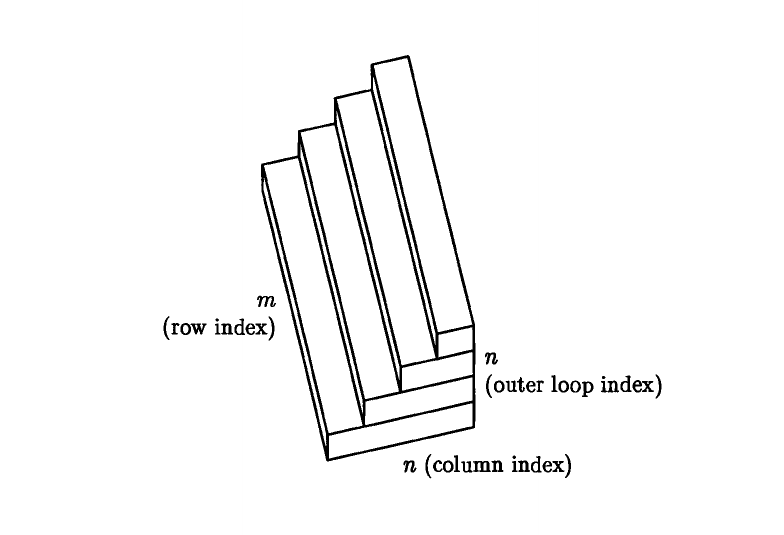
\includegraphics[width=0.62\linewidth]{../assets/figure-8-operation-count.png}
    \caption{修改后的 Gram--Schmidt 算法的运算量几何图示.底部的 $m\times n$ 矩形对应外层循环第一次遍历，向上的 $m\times(n-1)$ 矩形对应第二次遍历，依此类推.}
    \label{fig:operation-count}
\end{figure}

当 $m,n\to\infty$ 时，Gram--Schmidt 正交化的运算量与上图体积成正比.比例常数为 4 flops，因为内层循环的两步在每个矩阵位置各贡献约两次运算.图形趋近于体积为 $mn^2/2$ 的直三棱柱，因此再次得到
\begin{equation}
    \text{Gram--Schmidt 正交化的工作量}\sim 2mn^2\ \text{flops}.
    \tag{8.9}
\end{equation}
本书通常像式 (8.9) 这样记录运算量，而不把它们都写成定理.这类图除了帮助计算运算量，也提醒我们算法的结构.不同结构的算法图见原书第 75 页和第 176 页.

\section*{作为三角正交化的 Gram--Schmidt}

修改后的 Gram--Schmidt 算法的每一个外层步骤，都可以理解为在右侧乘一个方的上三角矩阵.例如，从 $A$ 开始，第一次迭代先把第一列 $a_1$ 乘以 $1/r_{11}$，再从其余各列 $a_j$ 中减去 $r_{1j}$ 倍的结果.这等价于右乘一个上三角矩阵 $R_1$；相应的原书结构图保留在图~\ref{fig:triangular-orthogonalization} 中.

一般而言，算法 8.1 的第 $i$ 步从当前矩阵的第 $j>i$ 列中减去 $r_{ij}/r_{ii}$ 倍的第 $i$ 列，并把第 $i$ 列替换为其 $1/r_{ii}$ 倍.这对应于右乘一个上三角矩阵 $R_i$.前几个矩阵的结构由图~\ref{fig:triangular-orthogonalization} 展示.

\begin{figure}[H]
    \centering
    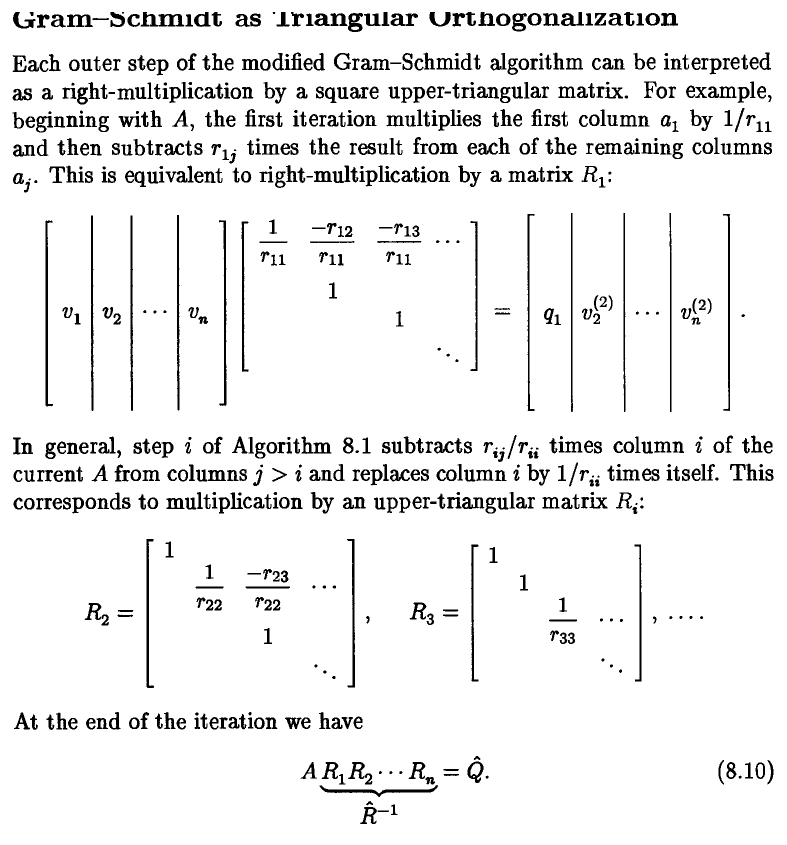
\includegraphics[width=0.96\linewidth]{../assets/figure-8-triangular-orthogonalization.png}
    \caption{把修改后的 Gram--Schmidt 迭代解释为右乘上三角矩阵.图中同时展示了 $R_1$、$R_2$、$R_3$ 的结构.}
    \label{fig:triangular-orthogonalization}
\end{figure}

迭代结束时有
\begin{equation}
    A R_1R_2\cdots R_n=\widehat Q,
    \qquad R_1R_2\cdots R_n=\widehat R^{-1}.
    \tag{8.10}
\end{equation}
这说明 Gram--Schmidt 算法确实是一种\textbf{三角正交化}.它在矩阵右侧施加三角运算，把矩阵化为列标准正交的矩阵.实际计算中我们当然不会显式形成 $R_i$ 并把它们相乘；引入这些矩阵的目的，是帮助理解算法结构.第 20 讲将看到，它与高斯消元的结构有密切相似之处.

\section*{习题}

\begin{enumerate}[label=\textbf{8.\arabic*}]
    \item 设 $A$ 是 $m\times n$ 矩阵.确定算法 8.1 计算 QR 分解 $A=\widehat Q\widehat R$ 时，浮点加法、减法、乘法和除法的精确次数.

    \item 编写 MATLAB 函数 `[Q,R]=mgs(A)`（见下一讲），用修改后的 Gram--Schmidt 正交化计算 $m\times n$ 矩阵 $A$ 的约化 QR 分解 $A=QR$，其中 $m\ge n$.输出变量是列标准正交的 $Q\in\C^{m\times n}$ 和三角矩阵 $R\in\C^{n\times n}$.

    \item 原书第 61 页的每个上三角矩阵 $R_i$ 都可以解释为一个对角矩阵与一个单位上三角矩阵（即对角元全为 1 的上三角矩阵）的乘积.准确说明这两个因子是什么，以及算法 8.1 的哪一行对应每个因子.
\end{enumerate}

\end{document}
